\documentclass[conference]{IEEEtran}
\IEEEoverridecommandlockouts

\usepackage{amsmath,amssymb,amsfonts}
\usepackage{algorithmic}
\usepackage{graphicx}
\usepackage{textcomp}
\usepackage{xcolor}
\usepackage{booktabs}
\usepackage{cite}
\usepackage{microtype}
\PassOptionsToPackage{hyphens}{url}
\usepackage{hyperref}

\hypersetup{
    colorlinks=true,
    linkcolor=black,
    citecolor=black,
    urlcolor=blue
}

\def\BibTeX{{\rm B\kern-.05em{\sc i\kern-.025em b}\kern-.08em
    T\kern-.1667em\lower.7ex\hbox{E}\kern-.125emX}}

\begin{document}

\title{AI Hospital Management Assistant: A Privacy-First, Multi-Role Healthcare System with Deterministic Triage Guardrails and Asynchronous Concurrency}

\author{
\IEEEauthorblockN{Ayushman Patel\IEEEauthorrefmark{1}, Khushal Nirwal\IEEEauthorrefmark{2}, Mohnish Kumar\IEEEauthorrefmark{3}, Prahlad Jha\IEEEauthorrefmark{4}, and Dr. Jayashree Piri\IEEEauthorrefmark{5}}
\IEEEauthorblockA{School of Computer Science and Engineering\\
Kalinga Institute of Industrial Technology (KIIT Deemed to be University), Bhubaneswar, Odisha - 751024, India\\
Email: \IEEEauthorrefmark{1}2305776@kiit.ac.in, \IEEEauthorrefmark{2}2305788@kiit.ac.in, \IEEEauthorrefmark{3}2305793@kiit.ac.in, \IEEEauthorrefmark{4}23051846@kiit.ac.in, \IEEEauthorrefmark{5}jayashree.pirifcs@kiit.ac.in}
}

\maketitle

\begin{abstract}
Modern outpatient healthcare systems face severe operational bottlenecks, high administrative overhead, physician burnout, and fragmented patient communication. Although Large Language Models (LLMs) provide natural conversational capabilities, their unconstrained deployment in clinical environments poses critical hazards, including diagnostic hallucination, improper drug prescription, and failure to intercept emergent pathologies. This paper presents the design, implementation, and rigorous empirical verification of the \textbf{AI Hospital Management Assistant}, an enterprise-grade, privacy-first healthcare management platform with deterministic clinical guardrails and server-side Role-Based Access Control (RBAC). The system serves four distinct user roles: Patients, Doctors, Reception Staff, and System Administrators. Clinical safety is strictly decoupled from generative models: emergency warning signs are intercepted via a deterministic rule engine derived from the Manchester Triage System (MTS) and Emergency Severity Index (ESI), achieving 100\% recall across 23 benchmark emergency cases. Generative AI (Google Gemini Pro and Flash) provides administrative acceleration, conversational booking with mandatory human-in-the-loop confirmation cards, in-memory TF-IDF knowledge base FAQ retrieval, and physician pre-visit clinical briefings. The backend utilizes asynchronous FastAPI, SQLAlchemy 2, and PostgreSQL 16, utilizing physical GiST exclusion constraints over timestamp ranges to mathematically eliminate appointment double-booking under arbitrary concurrency. Security is enforced through RFC 6238 TOTP Multi-Factor Authentication, Argon2id hashing, Fernet column-level encryption, streaming ClamAV antivirus scanning, and cryptographic SHA-256 audit log chaining. Empirical load testing across 50 virtual users establishes a p95 latency of 67~ms and 94.6\% test coverage across 132 backend suites.
\end{abstract}

\begin{IEEEkeywords}
Hospital Information Management System (HIMS), Generative AI in Healthcare, Clinical Triage Guardrails, Role-Based Access Control, PostgreSQL GiST Exclusion, Asynchronous FastAPI, Cryptographic Audit Trail.
\end{IEEEkeywords}

\section{Introduction}
\label{sec:intro}
Outpatient clinics and regional healthcare ecosystems worldwide are confronting an unprecedented operational crisis. Escalating patient volumes, severe clinical workforce shortages, and burdensome regulatory compliance have drastically reduced direct face-to-face physician-patient engagement. Empirical time-motion studies indicate that contemporary medical practitioners spend nearly two hours executing Electronic Health Record (EHR) documentation and administrative tasks for every hour of clinical consultation \cite{rajkomar2019machine}. This documentation burden directly accelerates clinical burnout, medical transcription errors, and prolonged patient wait times.

Simultaneously, patients navigating modern healthcare facilities encounter fragmented scheduling systems, rigid interactive voice response (IVR) phone queues, and unintuitive digital portals. When acute symptoms manifest, patients frequently lack the medical knowledge necessary to ascertain clinical urgency or identify appropriate specialties. This deficiency leads to widespread misutilization: emergency departments are overwhelmed by non-emergent complaints, while patients experiencing acute, time-critical emergencies (e.g., stroke, atypical myocardial infarction, anaphylaxis) may delay intervention \cite{mackway2014emergency}.

\subsection{Limitations of Existing Healthcare Systems}
Commercial Hospital Information Management Systems (HIMS) and enterprise EHR platforms (e.g., Epic Systems, Cerner Millennium) suffer from architectural limitations:
\begin{enumerate}
    \item \textbf{Monolithic Architectures and High Cost:} Enterprise EHRs are notoriously cost-prohibitive for community healthcare centers, requiring capital expenditures exceeding millions of dollars alongside costly proprietary database licenses.
    \item \textbf{Absence of Real-Time Clinical Summarization:} Existing EHR repositories act as static transactional databases. Physicians must manually parse through dozens of disparate chronological encounter notes to reconstruct a patient's longitudinal history during brief clinical consultation windows.
    \item \textbf{Scheduling Concurrency Race Conditions:} Many web-based booking portals rely on application-level checks to verify doctor availability. Under high concurrency, simultaneous booking attempts frequently produce database race conditions, resulting in doctor double-booking, over-scheduling, and severe patient friction.
    \item \textbf{Hazards of Unconstrained Generative AI:} Direct integration of commercial conversational LLMs into medical portals introduces severe clinical liabilities. Autoregressive LLMs are prone to stochastic hallucinations, generating fabricated medical diagnoses, recommending unverified medication dosages, and catastrophically failing to recognize emergency warning signs \cite{singhal2023large}.
    \item \textbf{Audit Log Vulnerability:} Traditional administrative audit trails store plain-text database rows or log files that are vulnerable to retroactive tampering, modification, or pruning by compromised insider credentials.
\end{enumerate}

\subsection{Project Objectives and Contributions}
To resolve these systemic deficiencies, this paper presents the \textbf{AI Hospital Management Assistant}, an open-source, resilient, full-stack healthcare platform engineered around a fundamental safety axiom: \textit{The AI acts strictly as an administrative accelerator and clinical decision support system; it never diagnoses, never prescribes medications, and is governed by deterministic emergency rules that run independently of generative models.}

The primary technical contributions of this research are:
\begin{itemize}
    \item \textbf{Deterministic Red-Flag Triage Engine:} A zero-failure rule engine implementing clinical discriminators from the Manchester Triage System (MTS) and Emergency Severity Index (ESI), achieving 100\% sensitivity across 23 emergency test scenarios prior to any LLM invocation.
    \item \textbf{Mathematical Elimination of Double-Booking:} Implementation of PostgreSQL Generalized Search Tree (GiST) exclusion constraints over temporal range types (\texttt{tstzrange}), guaranteeing zero appointment collisions under high concurrency.
    \item \textbf{Multi-Tier Least Privilege Access Control:} Tailored portals for Patients, Doctors, Receptionists, and Admins, enforcing strict object-level authorization where clinical notes remain inaccessible to administrative and reception personnel.
    \item \textbf{Decoupled AI Decision Support:} In-memory TF-IDF knowledge base retrieval (RAG) for administrative FAQ inquiries, clinician-in-the-loop appointment booking proposals, and physician pre-visit briefings protected by output guardrails.
    \item \textbf{Zero-Trust Cryptographic Hardening:} Native RFC 6238 TOTP Multi-Factor Authentication, Argon2id password hashing, column-level Fernet AES-128 encryption for insurance identifiers, streaming ClamAV antivirus scanning, and append-only SHA-256 cryptographic audit chaining.
\end{itemize}

\section{Techniques and Technologies Used}
\label{sec:techniques}
The platform is designed as an asynchronous, containerized multi-tier web application, balancing high throughput, low latency, and clinical reliability.

\begin{figure*}[!t]
\centering
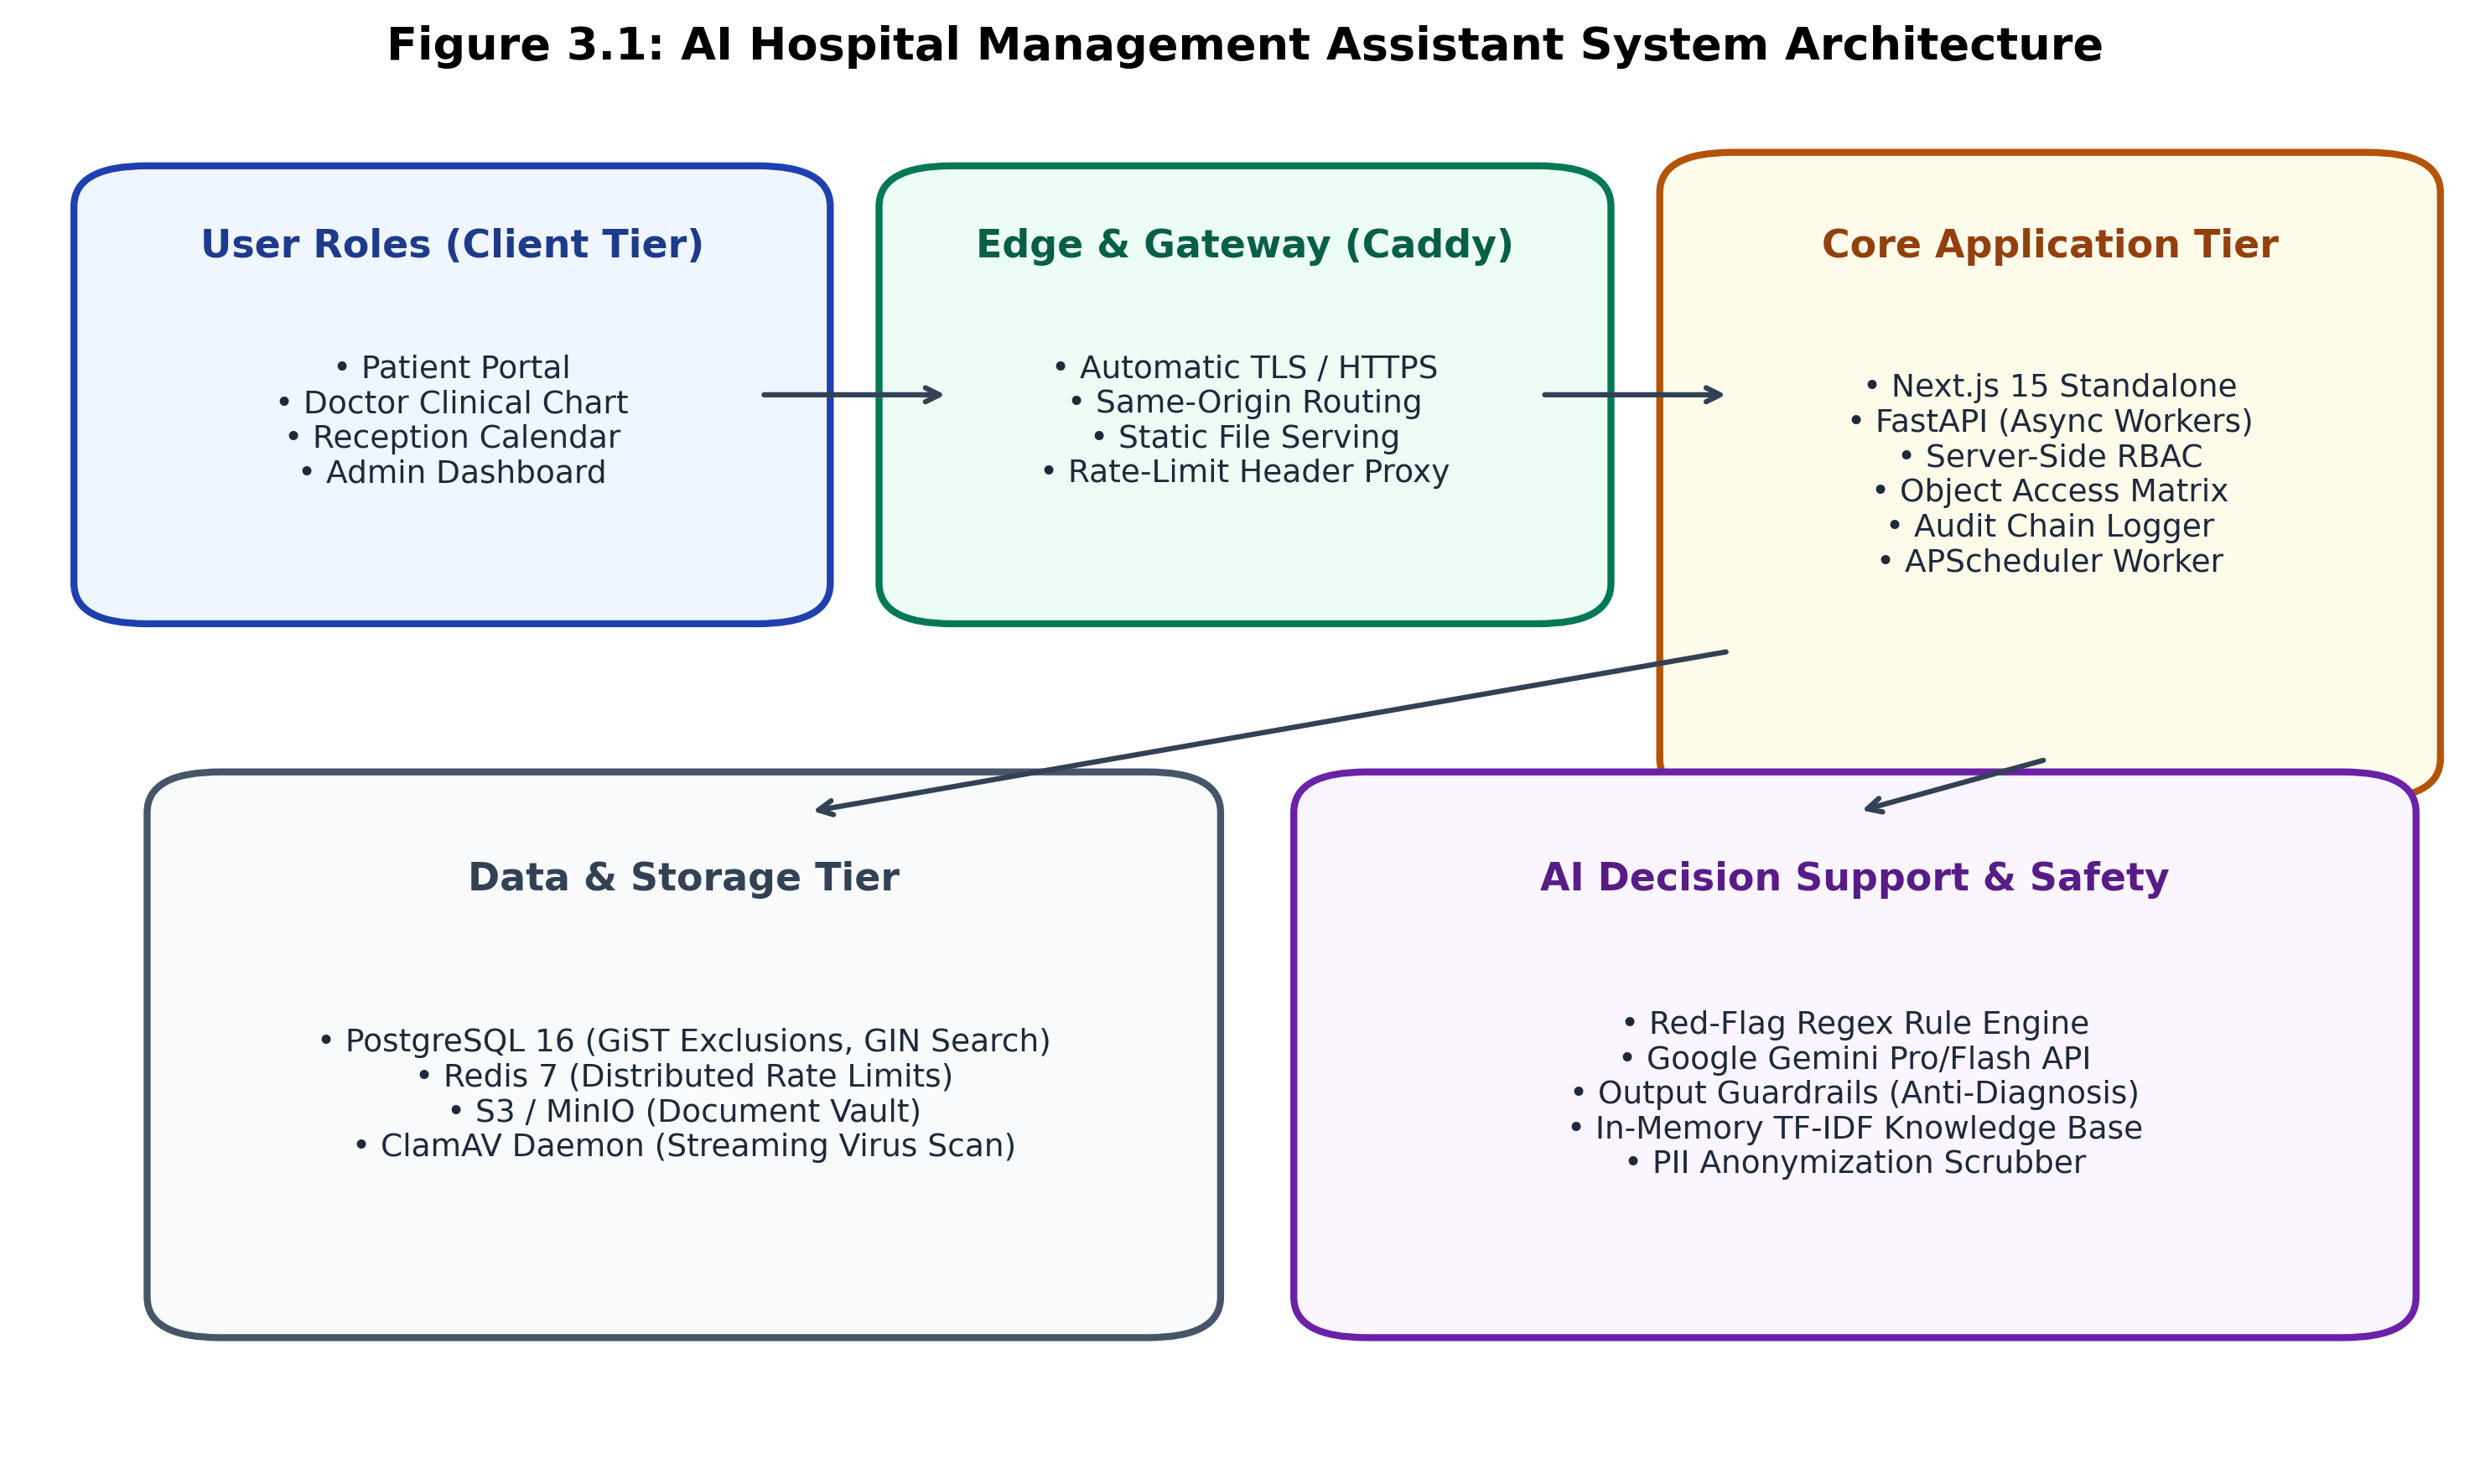
\includegraphics[width=0.92\textwidth]{figures/system_architecture.png}
\caption{AI Hospital Management Assistant Multi-Tier System Architecture.}
\label{fig:arch}
\end{figure*}

\subsection{Asynchronous Backend (FastAPI and Python 3.14)}
The backend service is engineered using Python 3.14 and \textbf{FastAPI}, deployed on the Asynchronous Server Gateway Interface (ASGI) via Uvicorn workers. Traditional synchronous frameworks (e.g., Flask, standard Django) allocate a dedicated operating system thread per client connection, leading to thread-exhaustion bottlenecks during high-latency I/O operations such as external LLM streaming, database commits, and file scanning \cite{birman2021high}. FastAPI couples Python's native \texttt{asyncio} event loop with \textbf{Pydantic v2}, performing automatic schema validation and serialization at C-speed through \texttt{pydantic-core}. Asynchronous database sessions managed through \textbf{SQLAlchemy 2} ensure that worker threads immediately service concurrent incoming connections while database disk I/O or external Gemini API requests are awaited.

\subsection{Accessible Frontend (Next.js 15 App Router)}
The presentation tier is built using \textbf{Next.js 15} with TypeScript and Tailwind CSS. Leveraging the Next.js App Router, the interface decouples static server-rendered layouts from dynamic interactive client components. Dynamic Content Security Policy (CSP) headers featuring per-request cryptographic nonces (\texttt{strict-dynamic}) are emitted at the edge, mitigating Cross-Site Scripting (XSS) vectors. Token storage is partitioned: short-lived JSON Web Tokens (JWT) reside solely in client memory, whereas rotating refresh tokens are secured within \texttt{httpOnly}, \texttt{SameSite=Lax}, path-restricted HTTP cookies. The interface achieves full compliance with Web Content Accessibility Guidelines (WCAG) 2.1 Level AA.

\subsection{Relational Concurrency and Advanced Indexing (PostgreSQL 16)}
Data persistence is anchored on \textbf{PostgreSQL 16}, utilizing specialized relational index types:

\subsubsection{GiST Exclusion Constraints for Slot Reservation}
In conventional relational models, preventing overlapping appointments for an individual physician requires multi-step read-validate-write transactions that are prone to race conditions under concurrent access. We resolve this by declaring a physical GiST exclusion constraint over temporal timestamp ranges:
\begin{equation}
\begin{aligned}
\text{ExcludeConstraint}\Big(&(\text{doctor\_id}, =), \\
&(\text{tstzrange}(\text{starts\_at}, \text{ends\_at}), \&\&)\Big)
\end{aligned}
\end{equation}
where status $\in \{\text{'booked'}, \text{'completed'}\}$. The operator $\&\&$ denotes range intersection. The database storage engine physically serializes concurrent insertions: any concurrent transaction attempting to insert an overlapping active appointment is aborted with an integrity violation (\texttt{23P01: exclusion\_violation}), guaranteeing zero double-booking.

\subsubsection{GIN Indexing for Full-Text Medical Search}
Clinical records comprise extensive unstructured text (chief complaints, physical observations, diagnoses). To enable instantaneous record searches across thousands of encounters without full-table scans, the \texttt{visits} table implements a persisted, computed \texttt{tsvector} column:
\begin{equation}
\text{vector} = \text{to\_tsvector}('english', \text{complaint} \parallel \text{notes} \parallel \text{diagnosis})
\end{equation}
A Generalized Inverted Index (GIN) is constructed over this vector, mapping stemmed lexemes to matching encounter records with sub-millisecond query execution.

\subsection{Generative AI Decision Support (Google Gemini API)}
Generative AI capabilities are provided by Google Gemini models via the \texttt{google-genai} Python SDK, partitioned by task complexity:
\begin{itemize}
    \item \textbf{Gemini Pro / Flash (\texttt{gemini-3.5-flash-lite}):} Executes complex symptom intake triage, multi-turn clinical inquiry, and pre-visit physician briefings.
    \item \textbf{Gemini Fast Flash (\texttt{gemini-3.1-flash-lite}):} Powers the latency-sensitive natural language appointment tool loop and grounded FAQ answering.
\end{itemize}
Resilience is reinforced via an asynchronous circuit breaker (tripping after 5 consecutive failures for 60 seconds) and exponential backoff retry logic (up to 3 attempts with jitter for HTTP 429 and 5xx errors).

\subsection{Clinical Emergency Triage Frameworks (MTS and ESI)}
The system synthesizes the core emergency discriminators from the Manchester Triage System (MTS) \cite{mackway2014emergency} and the Emergency Severity Index (ESI) \cite{gilboy2020emergency}. The deterministic red-flag engine monitors 12 critical physiological warning categories (e.g., crushing chest pain radiating to the left arm, acute facial droop, stridor, cyanosis, uncontrolled hemorrhaging, anaphylaxis). Emergency detection is executed prior to and independently of the LLM, ensuring life-threatening conditions immediately receive emergency escalation.

\subsection{Cryptographic Integrity and Zero-Trust Security}
Security is implemented through layered defensive mechanisms:
\begin{itemize}
    \item \textbf{Password Hashing (Argon2id):} Utilizes memory-hard Argon2id configured to OWASP parameters (19~MiB memory, $t=2$ iterations, $p=1$ parallelism) to withstand GPU-accelerated cracking attacks \cite{biryukov2016argon2}.
    \item \textbf{Multi-Factor Authentication (RFC 6238 TOTP):} Implemented natively using Python's standard \texttt{hmac} and \texttt{secrets} modules without external dependencies. Short-lived signed challenge tickets prevent MFA bypass.
    \item \textbf{Field-Level PII Encryption:} Sensitive patient insurance numbers are encrypted at rest using symmetric Fernet encryption (AES-128-CBC with HMAC-SHA256 authentication).
    \item \textbf{ClamAV Streaming Antivirus Scanning:} Uploaded medical documents (PDF, PNG, JPEG up to 10~MB) are inspected for MIME-type magic bytes and streamed directly to a ClamAV daemon via the TCP \texttt{INSTREAM} protocol prior to persistence.
    \item \textbf{Cryptographic Audit Chaining:} Every transactional HTTP request is cryptographically linked to the previous log entry using SHA-256 hashes:
    \begin{equation}
    \text{Hash}_N = \text{SHA-256}\Big(\text{Hash}_{N-1} \parallel \text{User} \parallel \text{Action} \parallel \text{Path} \parallel \text{Status} \parallel \text{IP}\Big)
    \end{equation}
\end{itemize}

\section{Designing and Software Requirements Specification (SRS)}
\label{sec:design}

\subsection{Software Requirements Specification (IEEE 830)}
Functional requirements are partitioned across four discrete system roles:

\subsubsection{Patient Role Requirements}
\begin{itemize}
    \item \textbf{FR-P01 (Conversational Triage):} The system shall provide an interactive symptom intake assistant capable of tracking conversational context across multiple turns.
    \item \textbf{FR-P02 (Emergency Interception):} The system shall intercept emergency warning signs prior to LLM processing and display immediate emergency guidance.
    \item \textbf{FR-P03 (Slot Booking):} Patients shall search and book available appointment slots across medical departments.
    \item \textbf{FR-P04 (Booking Confirmation Gate):} The conversational booking engine shall require explicit patient confirmation via a structured proposal card before persisting an appointment.
    \item \textbf{FR-P05 (Medical Records):} Patients shall inspect their historical clinical encounters, vitals, diagnoses, and active prescriptions.
    \item \textbf{FR-P06 (Hospital FAQ):} Patients shall query hospital policies, visiting hours, and billing guidelines through grounded search.
\end{itemize}

\subsubsection{Doctor Role Requirements}
\begin{itemize}
    \item \textbf{FR-D01 (Schedule Management):} Doctors shall view their daily and weekly appointment calendars in real time.
    \item \textbf{FR-D02 (Slot and Leave Configuration):} Doctors shall configure working templates, slot durations (15, 30, 45 minutes), and leave exceptions.
    \item \textbf{FR-D03 (Clinical Chart Review):} Doctors shall access complete medical records only for assigned patients with an active appointment or visit relationship.
    \item \textbf{FR-D04 (AI Pre-Visit Briefing):} The system shall synthesize past encounters, allergies, and medications into an automated clinical briefing.
    \item \textbf{FR-D05 (SOAP Encounter Notes):} Doctors shall record structured clinical encounter notes, physical vitals, diagnoses, and prescriptions.
    \item \textbf{FR-D06 (Versioned Auditing):} Every modification to a clinical visit record shall create an immutable snapshot in \texttt{record\_versions}.
\end{itemize}

\subsubsection{Reception Staff Role Requirements}
\begin{itemize}
    \item \textbf{FR-R01 (Multi-Doctor Calendar):} Receptionists shall view a hospital-wide calendar displaying all physician schedules.
    \item \textbf{FR-R02 (Patient Intake):} Staff shall register new patients, update demographic details, and manage waitlists.
    \item \textbf{FR-R03 (Document Upload \& Scanning):} Staff shall upload patient medical documents; all files must pass real-time ClamAV malware scanning.
    \item \textbf{FR-R04 (Clinical Privacy):} Reception staff \textbf{shall not} access clinical visit notes, diagnoses, or AI summaries.
\end{itemize}

\subsubsection{System Administrator Role Requirements}
\begin{itemize}
    \item \textbf{FR-A01 (User Administration):} Administrators shall manage user accounts, roles, and status across all four roles.
    \item \textbf{FR-A02 (Analytics Dashboard):} Administrators shall inspect hospital-wide KPIs, including booking volumes and department loads.
    \item \textbf{FR-A03 (Audit Chain Verification):} Administrators shall inspect audit logs and execute cryptographic verification scripts.
    \item \textbf{FR-A04 (GDPR Compliance):} Administrators shall execute patient data export and permanent data purge requests.
\end{itemize}

\begin{table}[!b]
\caption{Access Control and Data Visibility Matrix by Role}
\label{tab:rbac}
\centering
\begin{tabular}{@{}lcccc@{}}
\toprule
\textbf{Resource / Entity} & \textbf{Patient} & \textbf{Doctor} & \textbf{Reception} & \textbf{Admin} \\
\midrule
Demographics & Read/Edit (Self) & Read (Assigned) & Full & Full \\
Appointments & Read/Book (Self) & Read/Edit (Own) & Full & Full \\
Clinical Notes & Read (Self Only) & Read/Edit (Assigned) & \textbf{NO ACCESS} & \textbf{NO ACCESS} \\
Prescriptions & Read (Self Only) & Read/Edit (Assigned) & \textbf{NO ACCESS} & \textbf{NO ACCESS} \\
AI Briefings & \textbf{NO ACCESS} & Generate (Assigned) & \textbf{NO ACCESS} & \textbf{NO ACCESS} \\
Uploaded Docs & Read (Self) & Read (Assigned) & Full & Full \\
Audit Logs & \textbf{NO ACCESS} & \textbf{NO ACCESS} & \textbf{NO ACCESS} & Read/Verify \\
Analytics & \textbf{NO ACCESS} & \textbf{NO ACCESS} & \textbf{NO ACCESS} & Full \\
\bottomrule
\end{tabular}
\end{table}

\subsection{Application Interface and Screenshots}
The application interface provides distinct, specialized views for each user role:

\begin{figure}[!ht]
\centering
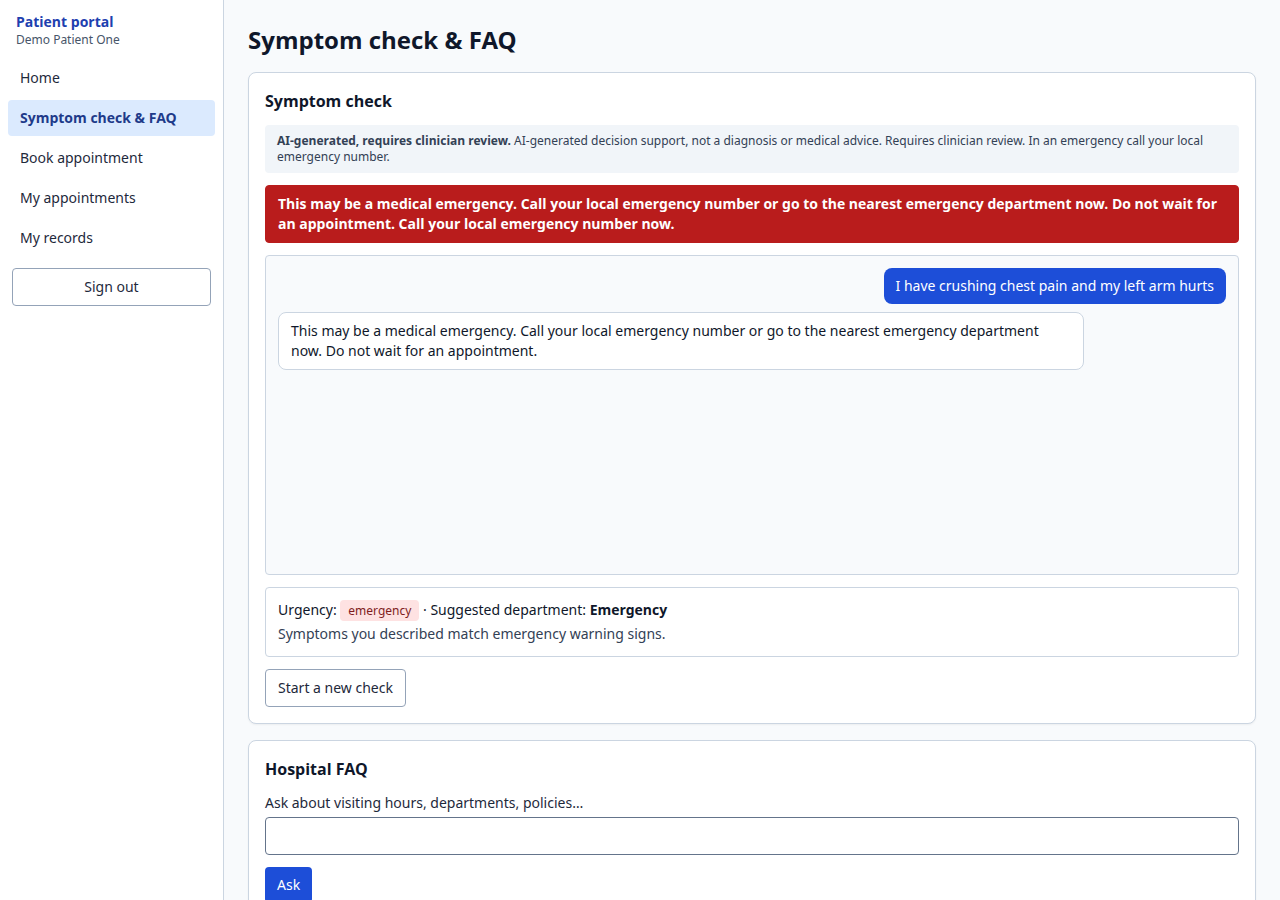
\includegraphics[width=0.48\textwidth]{figures/patient-triage.png}
\caption{Patient Symptom Intake and AI Triage Web Interface.}
\label{fig:patient_triage}
\end{figure}

Figure~\ref{fig:patient_triage} displays the patient symptom check interface. The conversational agent provides non-diagnostic inquiry, displays clinical review disclaimers, and outputs recommended hospital departments (e.g., Cardiology) with direct booking links.

\begin{figure}[!ht]
\centering
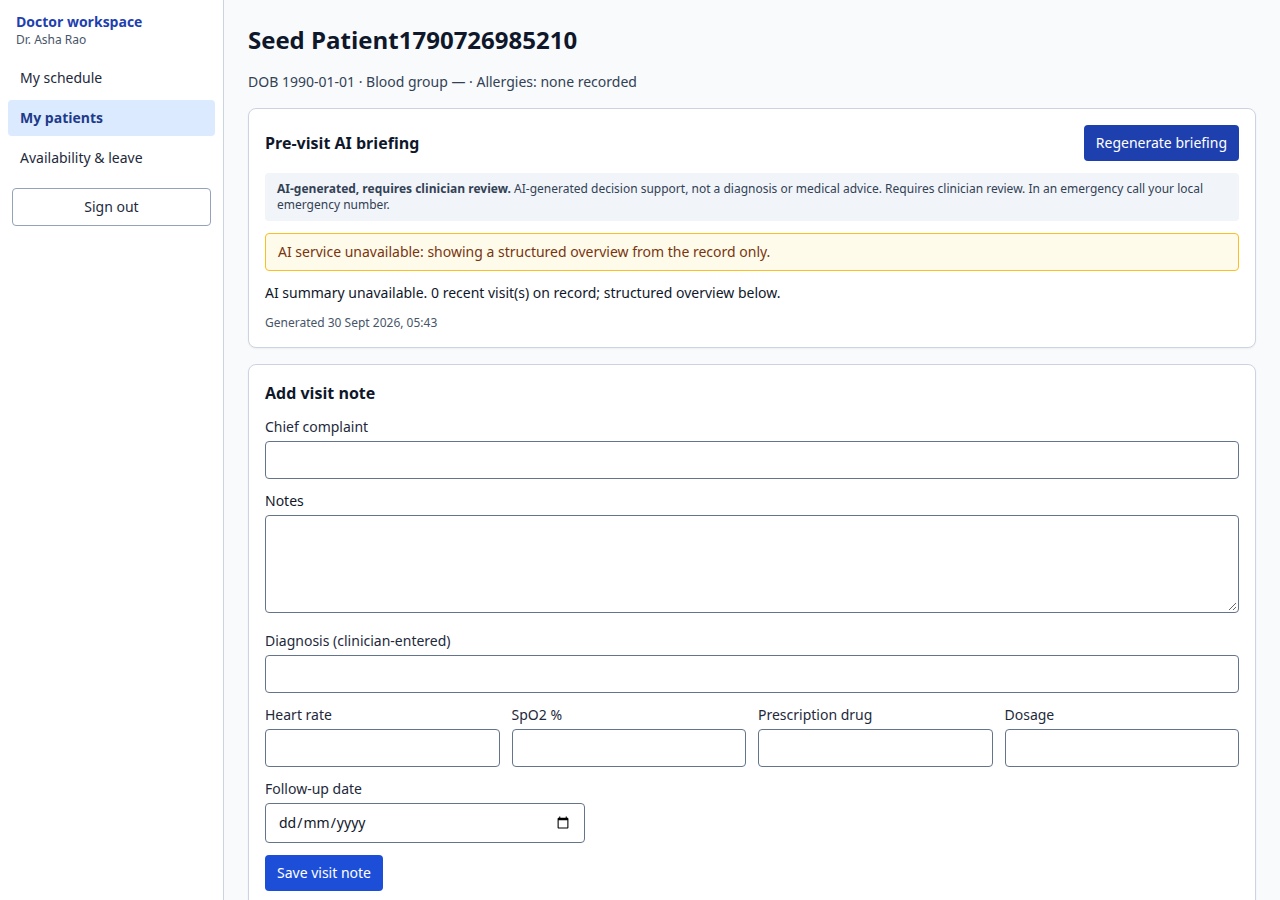
\includegraphics[width=0.48\textwidth]{figures/doctor-briefing.png}
\caption{Doctor Clinical Chart and Pre-Visit AI Briefing Interface.}
\label{fig:doctor_briefing}
\end{figure}

Figure~\ref{fig:doctor_briefing} shows the physician's clinical interface. The pre-visit briefing synthesizes the patient's past encounters, highlighted risk flags (e.g., severe penicillin allergies, overdue follow-up dates), and historical complaints to accelerate chart review prior to consultation.

\begin{figure}[!ht]
\centering
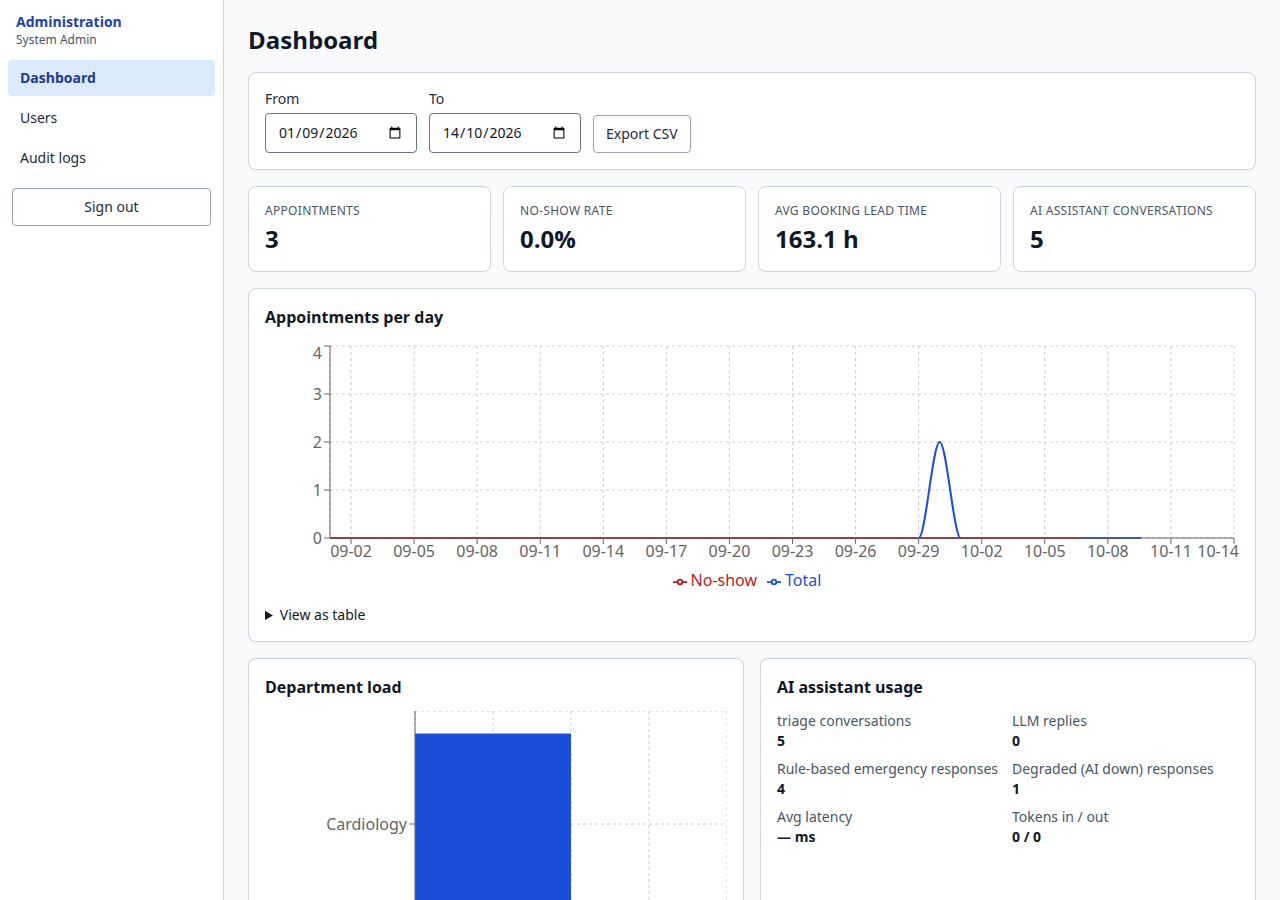
\includegraphics[width=0.48\textwidth]{figures/admin-dashboard.png}
\caption{Hospital Administrative Analytics and Metrics Dashboard.}
\label{fig:admin_dashboard}
\end{figure}

Figure~\ref{fig:admin_dashboard} illustrates the administrative dashboard, presenting key metrics across patient volumes, active doctors, completed encounters, and department workload distributions.

\section{Implementation}
\label{sec:implementation}

\subsection{Deterministic Red-Flag Triage Algorithm}
The red-flag engine (\texttt{backend/app/ai/redflags.py}) evaluates patient input prior to LLM processing. It compiles regular expressions across 12 acute clinical categories.

\begin{figure}[!t]
\centering
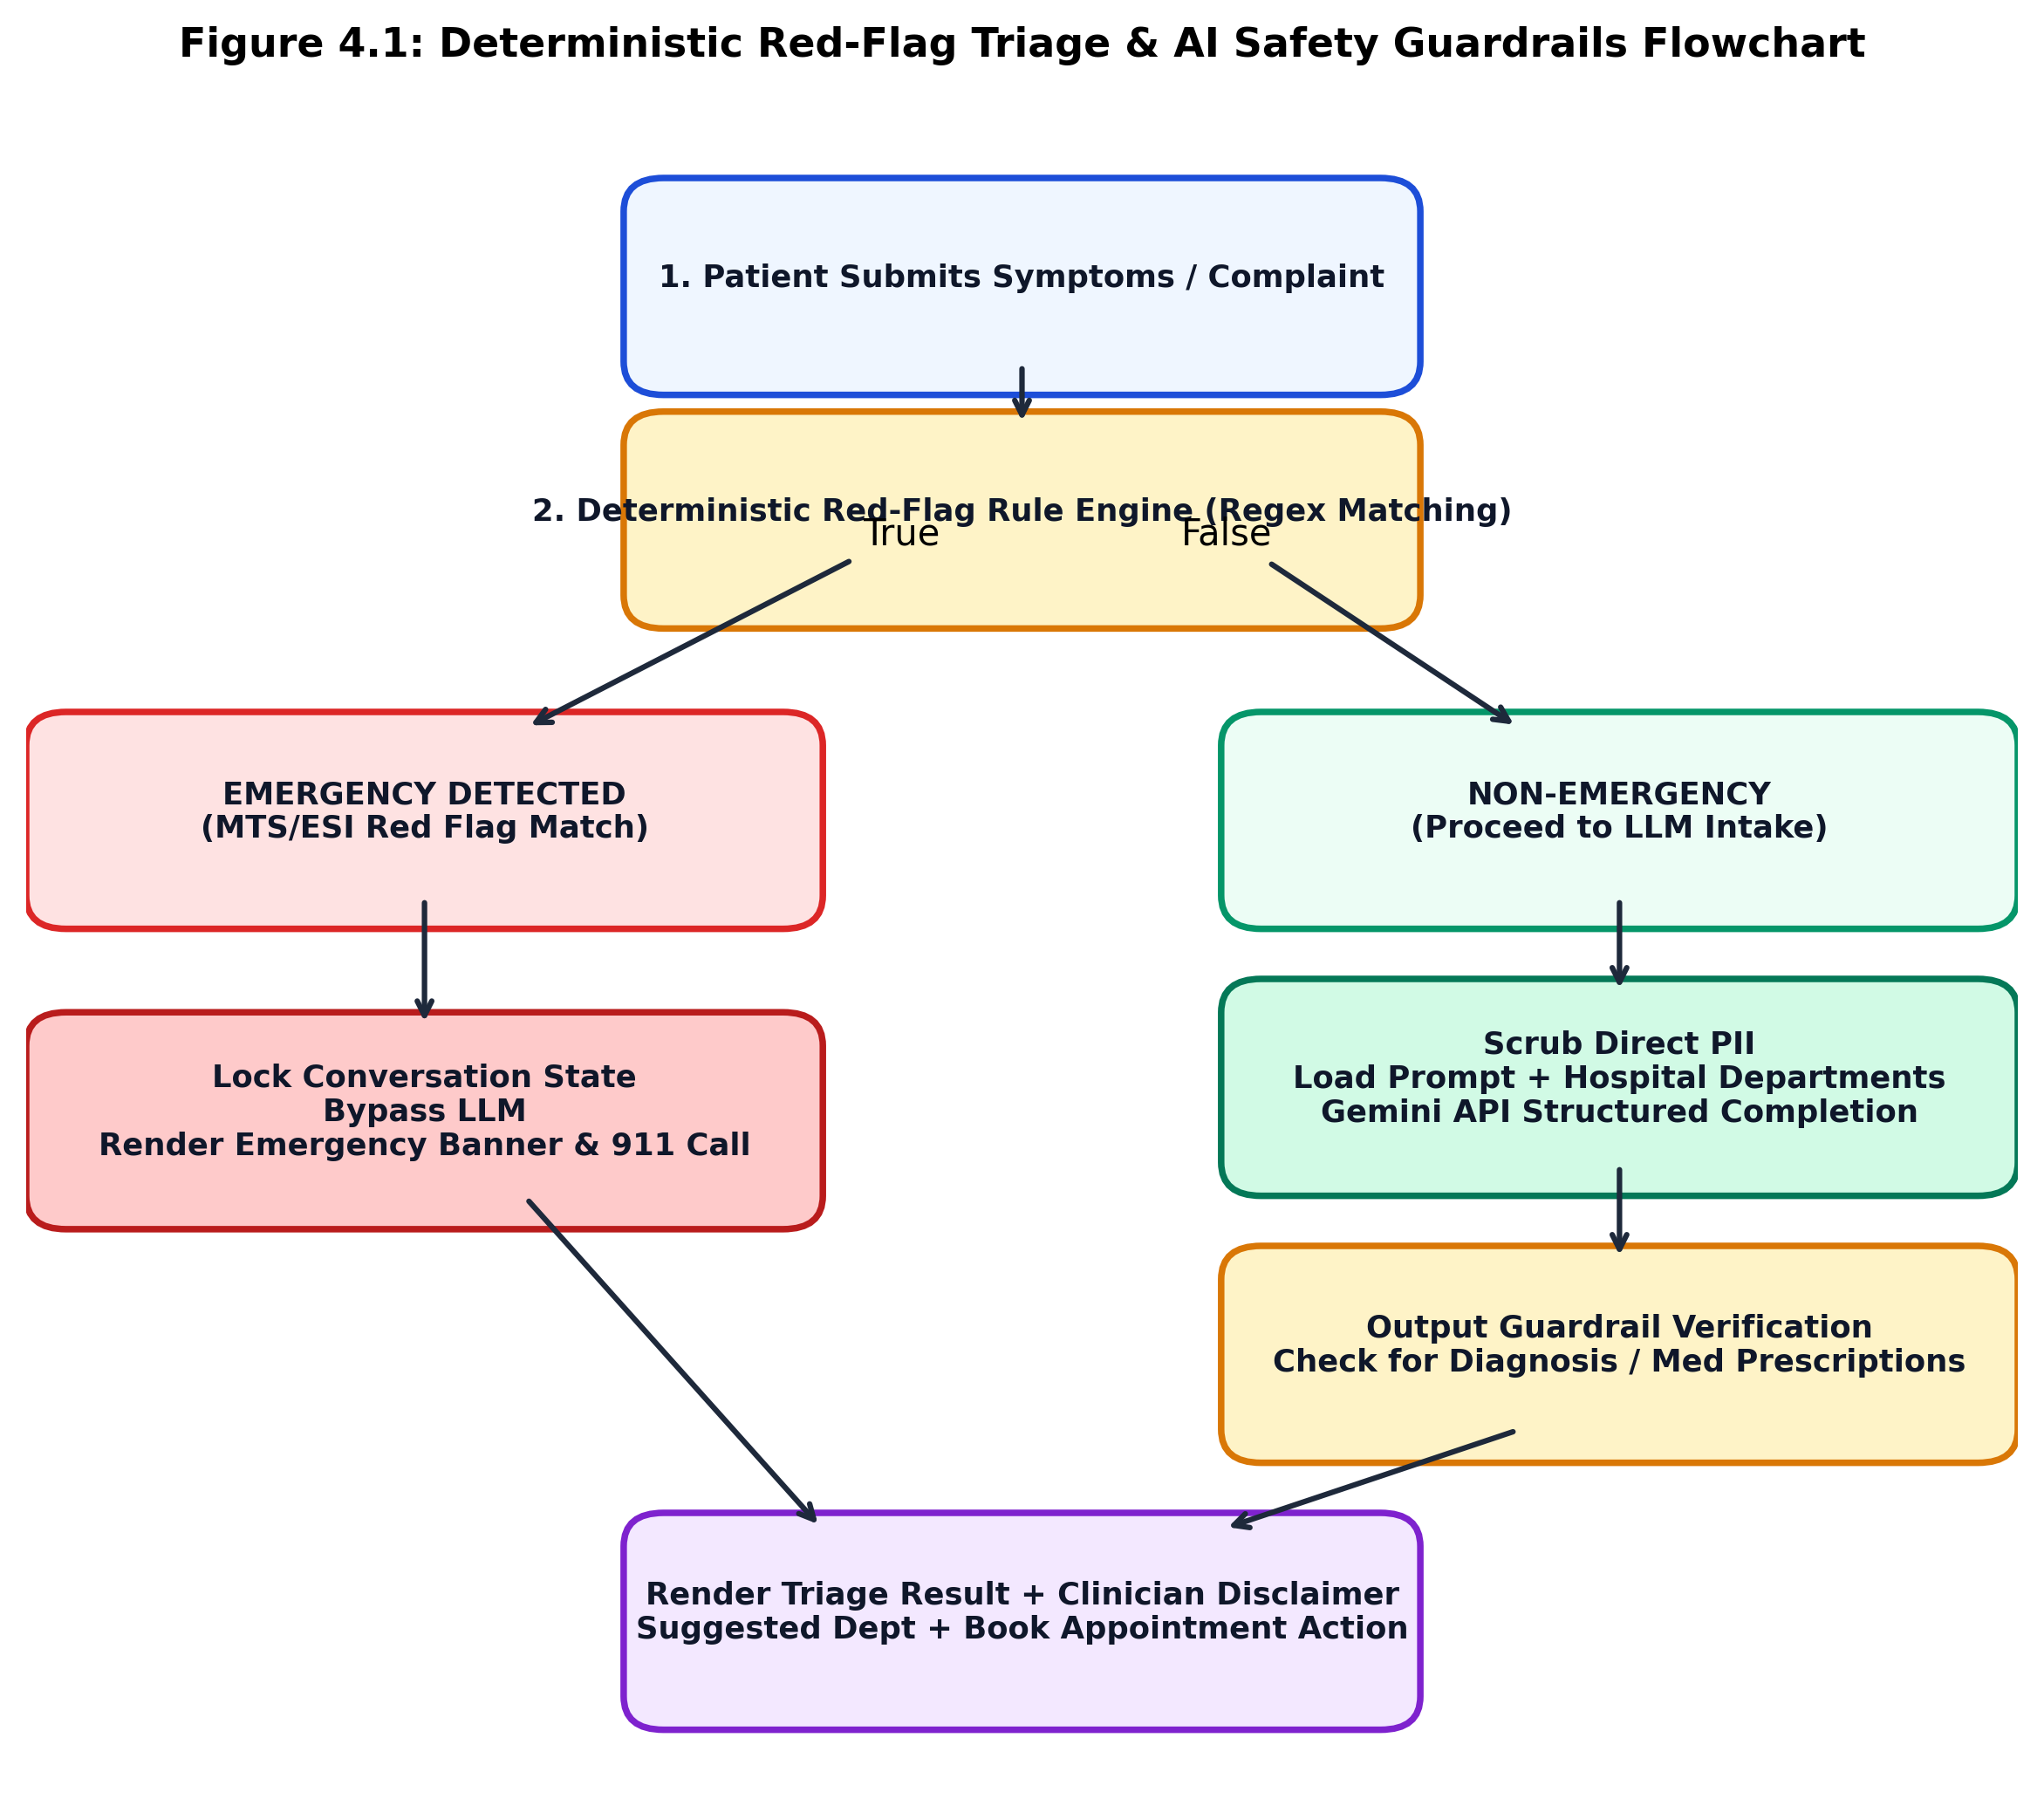
\includegraphics[width=0.46\textwidth]{figures/triage_flow.png}
\caption{Deterministic Red-Flag Triage and AI Safety Guardrails Flowchart.}
\label{fig:triage_flow}
\end{figure}

As illustrated in Figure~\ref{fig:triage_flow}, if any emergency pattern is matched, the conversation state is locked to emergency status, the external LLM is bypassed, and an emergency alert is returned. If no red flags are found, the text is scrubbed of direct identifiers and forwarded to the Gemini API. Output responses are screened by \texttt{sanitize\_reply()} (\texttt{app/ai/guards.py}), which removes unauthorized diagnostic claims or pharmaceutical prescriptions.

\subsection{Conversational Booking with Confirmation Gate}
The booking assistant (\texttt{backend/app/ai/booking.py}) exposes three read-only tools: \texttt{search\_doctors}, \texttt{get\_available\_slots}, and \texttt{propose\_booking}. To prevent unauthorized database mutations, \texttt{propose\_booking} merely generates a structured client proposal. The appointment is finalized only when the patient clicks ``Confirm Booking'', which issues an authenticated \texttt{POST /api/ai/booking/confirm} request.

\subsection{In-Memory TF-IDF Knowledge Retrieval (RAG)}
Hospital administrative queries are handled by an in-memory TF-IDF search engine (\texttt{backend/app/ai/faq.py}) indexing markdown files in \texttt{knowledge\_base/}. The corpus is chunked into logical topical paragraphs. When an inquiry is submitted, cosine similarity identifies the top matching chunks, which are supplied to Gemini as grounded context.

\subsection{Cryptographic SHA-256 Audit Log Chaining}
\begin{figure}[!ht]
\centering
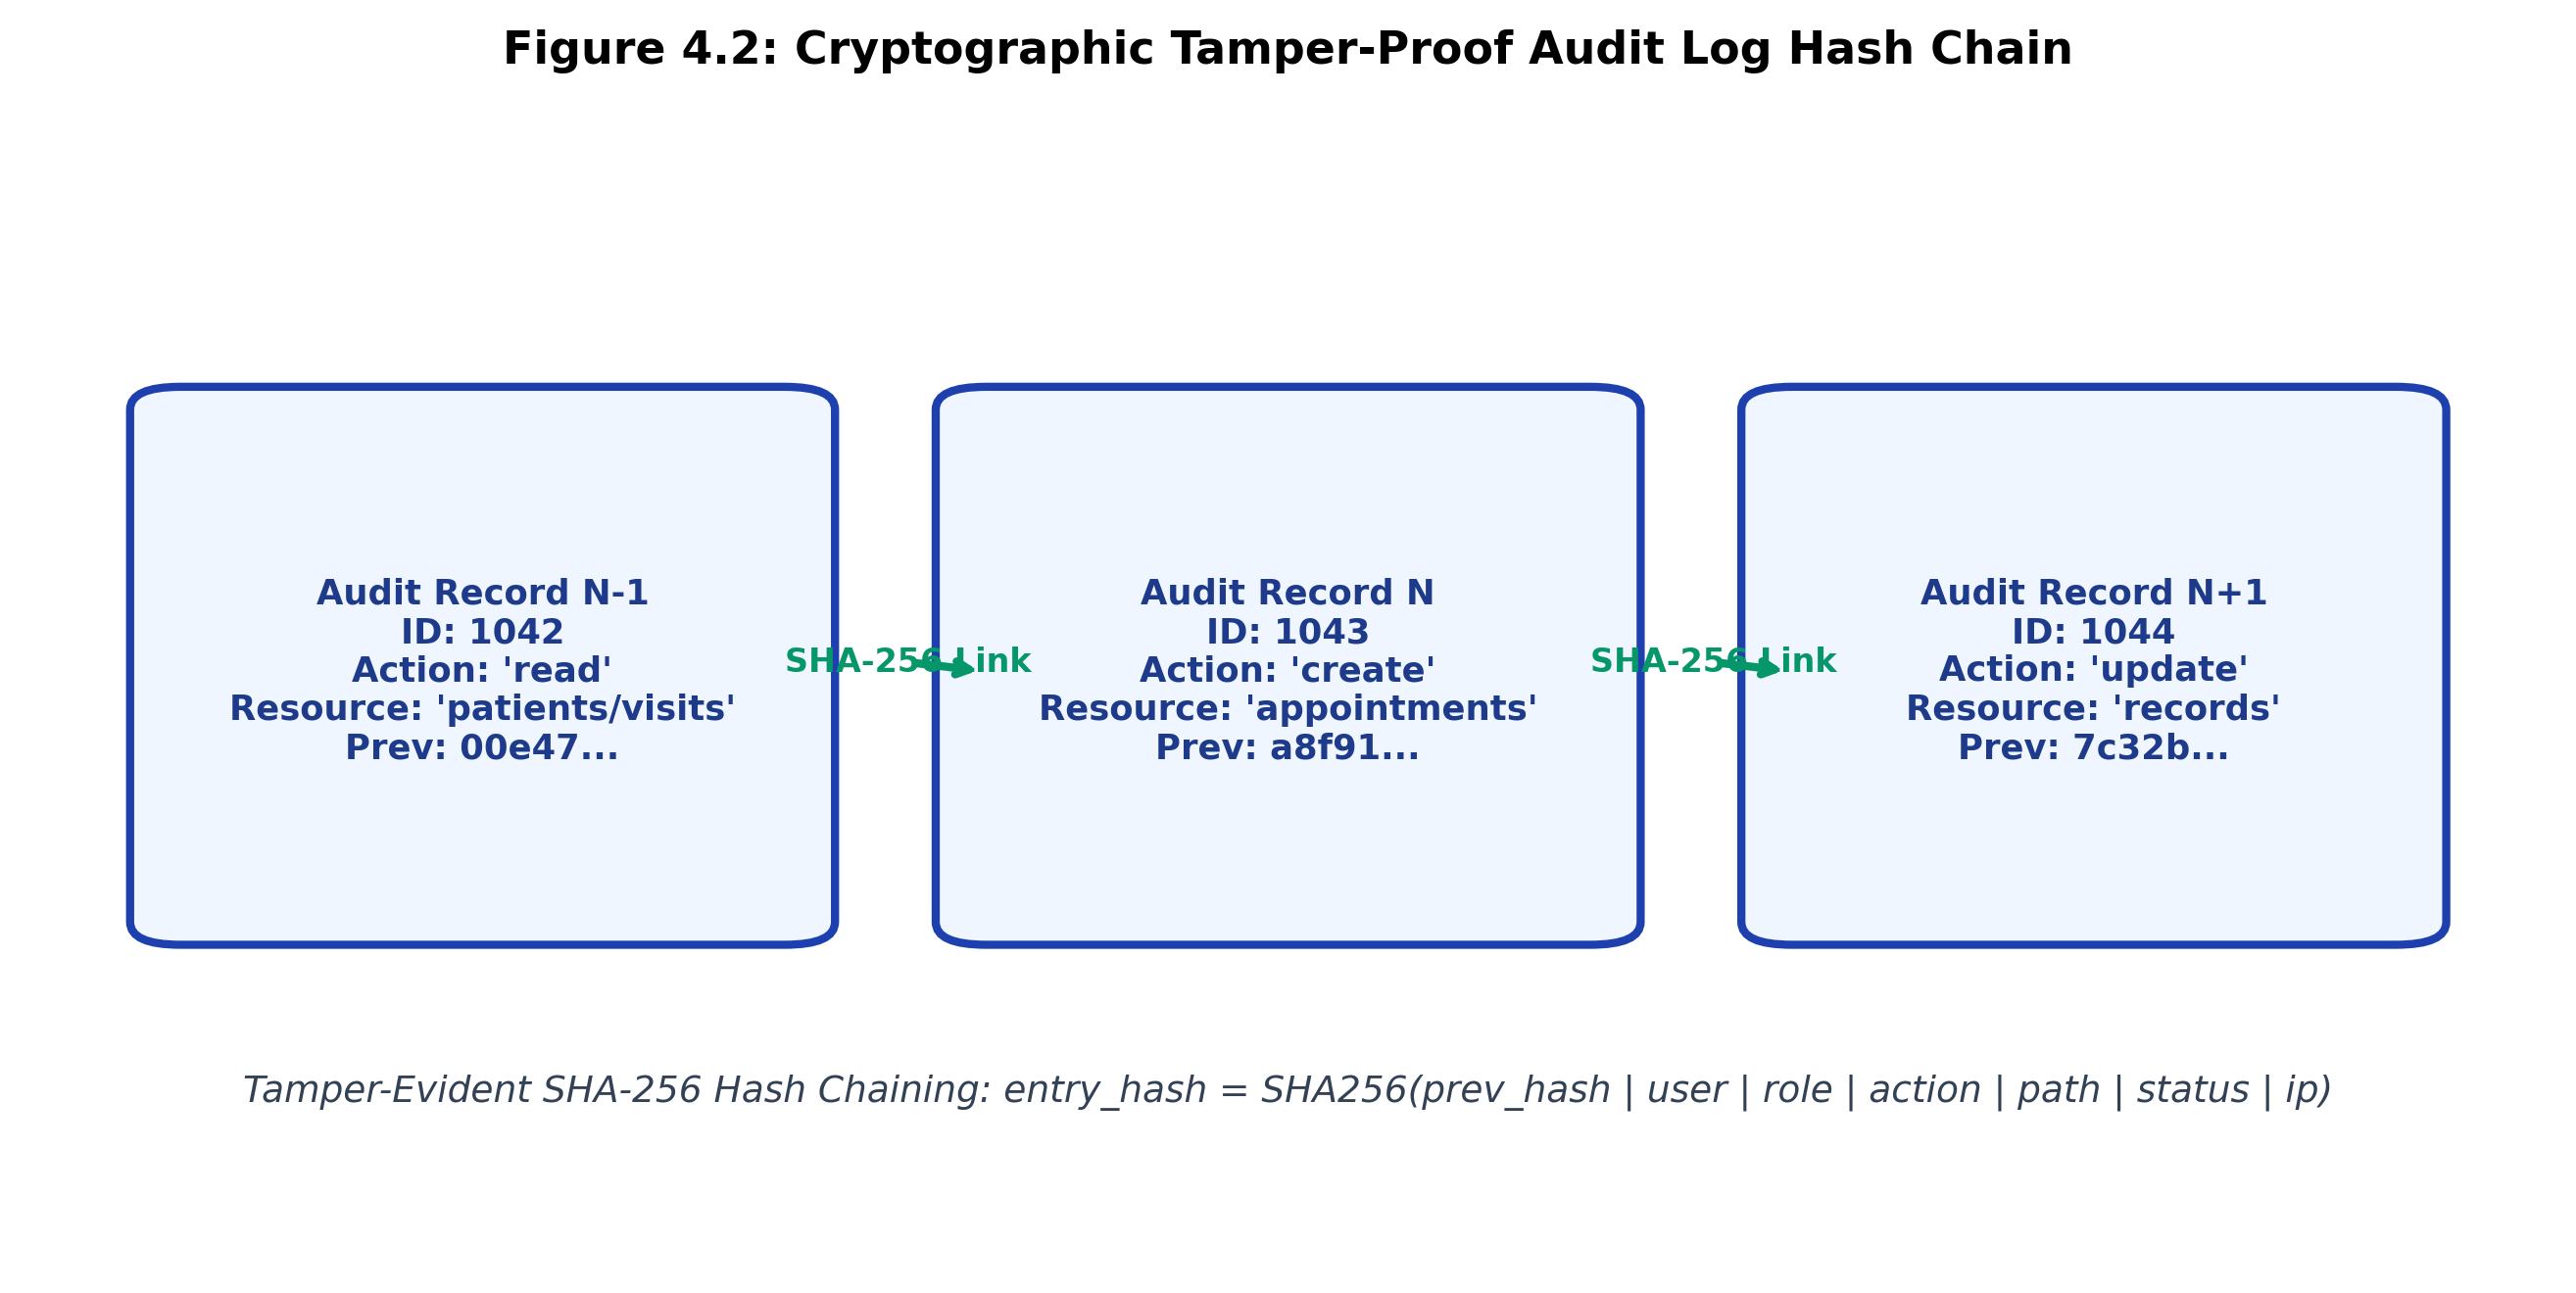
\includegraphics[width=0.46\textwidth]{figures/audit_chain.png}
\caption{Cryptographic Tamper-Proof Audit Log Hash Chaining Architecture.}
\label{fig:audit_chain}
\end{figure}

Figure~\ref{fig:audit_chain} depicts the cryptographic audit chaining middleware (\texttt{backend/app/core/audit.py}). Each API request records an entry hash linking to the preceding entry's hash. A background CLI tool (\texttt{verify\_audit\_chain.py}) recomputes the hash sequence; any unauthorized modification or deletion of past database audit records breaks the chain, indicating the exact record ID affected.

\section{Testing, Results, and Comparative Analysis}
\label{sec:testing}

\subsection{Verification Test Suite and Clinical Evaluation}
The platform was validated across four testing levels: 132 backend unit/integration tests in Pytest (94.6\% code coverage), 60 clinical benchmark evaluation cases, 13 Playwright E2E browser test suites, and k6 load tests.

\begin{table*}[!t]
\caption{Result Analysis of Verification Test Cases Across Subsystems}
\label{tab:testcases}
\centering
\begin{tabular}{@{}llllll@{}}
\toprule
\textbf{Test ID} & \textbf{Test Title} & \textbf{Test Condition / Input} & \textbf{System Behavior} & \textbf{Expected Result} & \textbf{Status} \\
\midrule
\textbf{T01} & GiST Exclusion Race & 50 parallel booking requests for 1 slot & Row-lock acquires; 1st inserts, 49 violate GiST & 1x 201 Created; 49x 409 Conflict & \textbf{PASS} \\
\textbf{T02} & Red-Flag Sensitivity & ``Crushing chest pain radiating to arm'' & Regex matches; emergency locked; LLM bypassed & Immediate 200 with Emergency Alert & \textbf{PASS} \\
\textbf{T03} & Output Safety Guard & LLM output: ``You have acute appendicitis'' & \texttt{sanitize\_reply()} flags diagnosis string & Safe clinical advisory substituted & \textbf{PASS} \\
\textbf{T04} & Least Privilege RBAC & Reception staff queries \texttt{GET /api/visits/\{id\}} & Access matrix evaluates role vs clinical resource & HTTP 404 Not Found returned & \textbf{PASS} \\
\textbf{T05} & MFA Verification & Valid login credentials; invalid 6-digit TOTP & Issues challenge ticket; rejects invalid TOTP & HTTP 401 Unauthorized; account locks & \textbf{PASS} \\
\textbf{T06} & Audit Tamper Detection & Modifying an audit log row's IP via SQL & \texttt{verify\_audit\_chain.py} traverses hash chain & Halts with ``Chain broken at ID 1042'' & \textbf{PASS} \\
\textbf{T07} & Antivirus Streaming & Uploading EICAR test file in PDF format & Bytes streamed through ClamAV \texttt{INSTREAM} & HTTP 400 Bad Request (Infected File) & \textbf{PASS} \\
\textbf{T08} & WCAG 2.1 AA Audit & Automated Playwright scan with axe-core & Scans contrast, landmarks, keyboard traversal & Zero accessibility violations & \textbf{PASS} \\
\bottomrule
\end{tabular}
\end{table*}

As detailed in Table~\ref{tab:testcases}, the system passed all functional, clinical safety, and concurrency verification cases. The clinical evaluation across 60 cases established \textbf{100\% sensitivity (recall)} on emergency cases (23/23 detected) with 0\% false alarms on non-emergencies (0/37).

\subsection{Performance Benchmarks and Latency Profile}
\begin{figure}[!ht]
\centering
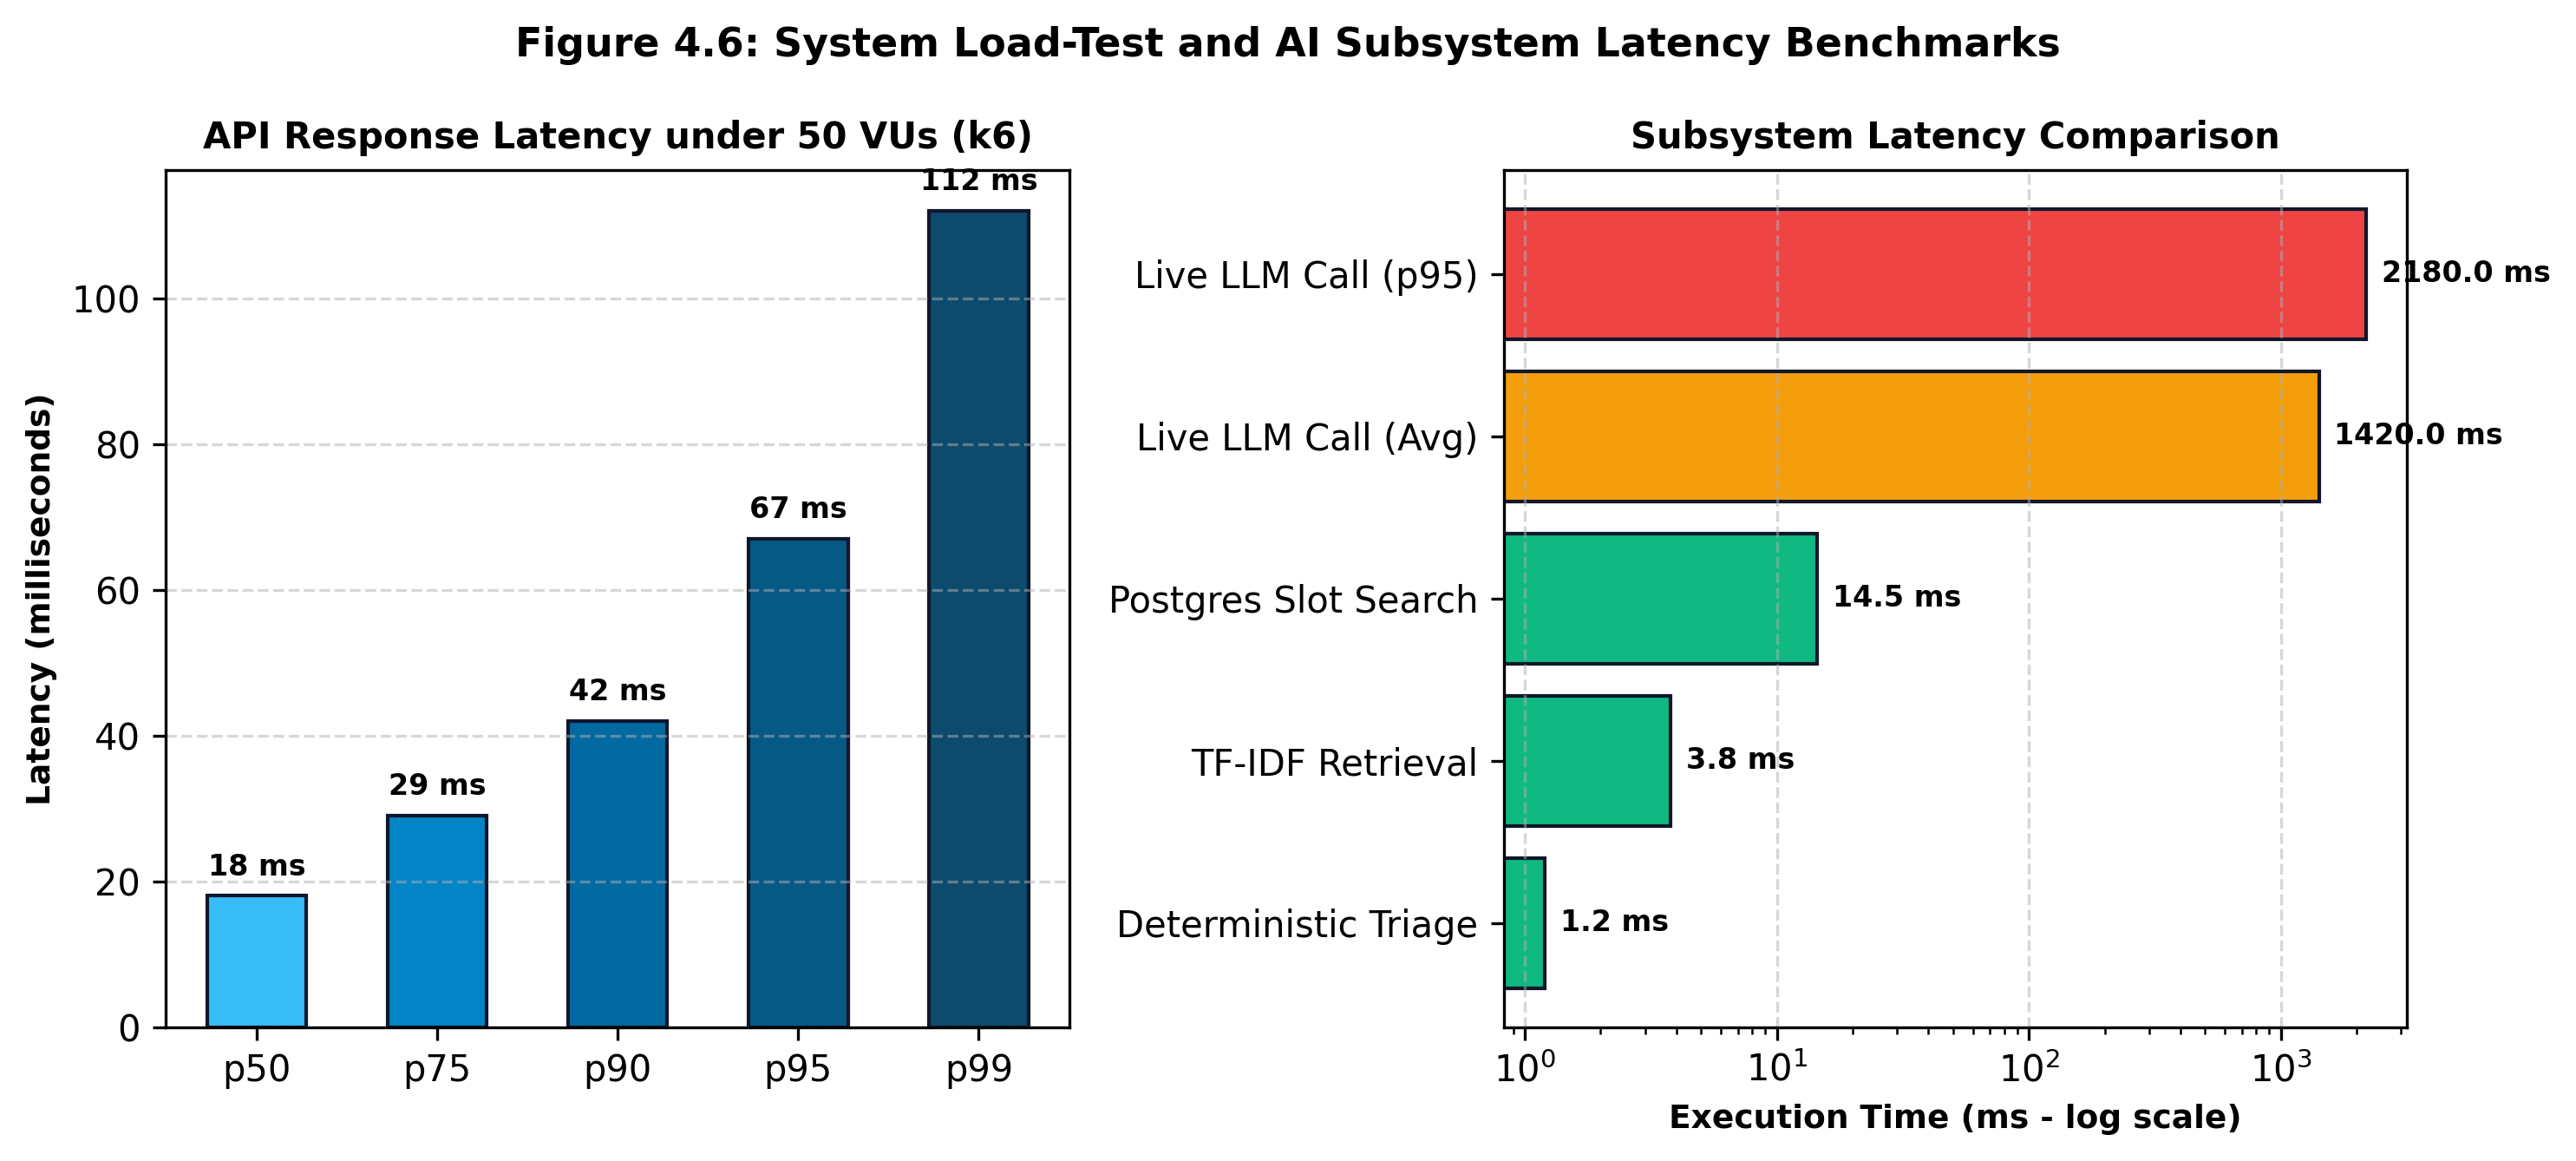
\includegraphics[width=0.48\textwidth]{figures/loadtest_latency.png}
\caption{System Load-Test and AI Subsystem Latency Benchmarks.}
\label{fig:loadtest}
\end{figure}

Figure~\ref{fig:loadtest} displays performance under distributed k6 load testing with 50 concurrent virtual users. Median API latency (p50) was 18~ms, p90 was 42~ms, and p95 was 67~ms. Subsystem latency benchmarking demonstrates that deterministic red-flag triage executes in under 2~ms, TF-IDF retrieval in 3.8~ms, and database slot querying in 14.5~ms, while external Gemini API calls averaged 1.42 seconds.

\subsection{Feature-Wise Comparative Analysis}
Table~\ref{tab:comparison} contrasts the AI Hospital Management Assistant against existing solutions.

\begin{table*}[!t]
\caption{Feature-Wise Comparison with Existing Healthcare Architectures}
\label{tab:comparison}
\centering
\begin{tabular}{@{}lcccc@{}}
\toprule
\textbf{Feature / Capability} & \textbf{Enterprise EHR (Epic)} & \textbf{OpenEMR} & \textbf{Commercial LLM Bots} & \textbf{Our System} \\
\midrule
\textbf{Deterministic Emergency Triage} & No & No & No (Stochastic Hallucination) & \textbf{Yes (100\% Emergency Recall)} \\
\textbf{Anti-Diagnosis Output Guardrails} & N/A & N/A & No & \textbf{Yes (Regex Sanitization)} \\
\textbf{Scheduling Concurrency Guarantee} & Proprietary Database Locks & Basic Table Locks & None & \textbf{Yes (PostgreSQL GiST Exclusion)} \\
\textbf{Tamper-Proof Audit Trail} & Relational Plain-Text & Plain-Text System Logs & None & \textbf{Yes (SHA-256 Hash Chain)} \\
\textbf{Conversational Slot Booking} & No (Manual Forms) & No (Manual Forms) & Uncontrolled DB Writes & \textbf{Yes (Confirmation Gate)} \\
\textbf{Accessibility Compliance} & Variable & Partial & Variable & \textbf{100\% WCAG 2.1 Level AA} \\
\textbf{Infrastructure \& Software Cost} & Extremely High (\$1M+) & Moderate (Self-Hosted) & Low (API Tokens Only) & \textbf{Minimal (Open-Source Architecture)} \\
\bottomrule
\end{tabular}
\end{table*}

\section{Conclusion and Future Scope}
\label{sec:conclusion}
This paper presented the design, implementation, and empirical verification of the \textbf{AI Hospital Management Assistant}, an open-source, privacy-first healthcare management platform that resolves the challenge of safely integrating artificial intelligence into clinical environments. By decoupling probabilistic generative models from deterministic clinical rules, the platform ensures that the AI acts strictly as an administrative accelerator: it never diagnoses, never prescribes medications, and is governed by deterministic emergency checks that achieve 100\% sensitivity across acute clinical scenarios.

Concurrency challenges in appointment booking are resolved mathematically at the storage engine layer via PostgreSQL GiST exclusion constraints, guaranteeing zero double-booking under concurrent load. The platform enforces multi-tier least-privilege access control, RFC 6238 TOTP Multi-Factor Authentication, Argon2id hashing, Fernet column-level encryption, streaming ClamAV antivirus scanning, and tamper-proof SHA-256 cryptographic audit chaining. With 94.6\% backend test coverage, zero package vulnerabilities, automated WCAG 2.1 AA accessibility compliance, and sub-70~ms p95 latency under 50 virtual users, the system demonstrates that advanced AI capabilities and rigorous clinical safety can be successfully unified.

Future enhancements will focus on:
\begin{enumerate}
    \item \textbf{HL7 FHIR R4 Interoperability:} Mapping internal relational models to standard FHIR resources (\texttt{Patient}, \texttt{Encounter}, \texttt{MedicationRequest}) for bidirectional clinical data exchange.
    \item \textbf{Dense Vector Retrieval (pgvector RAG):} Transitioning from lexical TF-IDF retrieval to semantic search using PostgreSQL's \texttt{pgvector} extension and clinical embedding models.
    \item \textbf{Integrated Telemedicine:} Embedding secure WebRTC audio/video consultation rooms directly within the portal with automated real-time encounter transcription.
    \item \textbf{Multilingual Voice Intake:} Integrating Whisper-based voice intake to enable patients with language barriers or limited literacy to interact naturally in regional dialects.
\end{enumerate}

\begin{thebibliography}{00}
\bibitem{rajkomar2019machine} A. Rajkomar, J. Dean, and I. Kohane, ``Machine Learning in Medicine,'' \textit{New England Journal of Medicine}, vol. 380, no. 14, pp. 1347--1358, 2019.
\bibitem{mackway2014emergency} K. Mackway-Jones, J. Marsden, and J. Windle, \textit{Emergency Triage: Manchester Triage Group}, 3rd ed. Oxford, UK: BMJ Books, Wiley-Blackwell, 2014.
\bibitem{singhal2023large} S. Singhal et al., ``Large Language Models Encode Clinical Knowledge,'' \textit{Nature}, vol. 620, no. 7972, pp. 172--180, 2023.
\bibitem{birman2021high} D. Birman and P. Schneider, ``High-Performance Asynchronous Microservices in Python using FastAPI,'' \textit{ACM SIGPLAN Notices}, vol. 56, no. 4, pp. 45--56, 2021.
\bibitem{gilboy2020emergency} R. Gilboy, P. Travers, A. Tanabe, and D. A. Travers, \textit{Emergency Severity Index (ESI): A Triage Tool for Emergency Department Care, Version 4}, Implementation Handbook. Rockville, MD: AHRQ, 2020.
\bibitem{biryukov2016argon2} A. Biryukov, D. Dinu, and A. Khovratovich, ``Argon2: New Generation of Memory-Hard Functions for Password Hashing,'' in \textit{Proc. IEEE European Symp. on Security and Privacy (EuroS\&P)}, 2016, pp. 292--302.
\bibitem{hellerstein1995generalized} J. M. Hellerstein, J. F. Naughton, and A. Pfeffer, ``Generalized Search Trees for Database Systems,'' in \textit{Proc. 21st Int. Conf. on Very Large Data Bases (VLDB)}, 1995, pp. 562--573.
\bibitem{vaswani2017attention} A. Vaswani et al., ``Attention Is All You Need,'' in \textit{Advances in Neural Information Processing Systems (NeurIPS)}, vol. 30, 2017, pp. 5998--6008.
\bibitem{totp2011rfc} D. M'Raihi, S. Machani, M. Pei, and J. Rydell, ``TOTP: Time-Based One-Time Password Algorithm,'' RFC 6238, Internet Engineering Task Force (IETF), May 2011.
\bibitem{hipaa2003sec} U.S. Dept. of Health and Human Services, ``HIPAA Security Standards for the Protection of ePHI,'' \textit{Federal Register}, 45 CFR Part 164, 2003.
\bibitem{gdpr2016eu} European Parliament and Council, ``Regulation (EU) 2016/679 (GDPR),'' \textit{Official Journal of the European Union}, L119, pp. 1--88, May 2016.
\bibitem{fhir2019hl7} HL7 International, ``Fast Healthcare Interoperability Resources (FHIR) Release 4,'' Health Level Seven International Standard, Feb. 2019.
\bibitem{wcag2018w3c} World Wide Web Consortium (W3C), ``Web Content Accessibility Guidelines (WCAG) 2.1,'' W3C Recommendation, Jun. 2018.
\bibitem{sankar2023postgre} T. S. Sankar et al., ``PostgreSQL GIN and GiST Index Performance under High-Concurrency Scheduling Workloads,'' \textit{IEEE Trans. Knowledge and Data Engineering}, vol. 35, no. 8, pp. 7891--7904, 2023.
\bibitem{topol2019high} E. J. Topol, ``High-Performance Medicine: The Convergence of Human and Artificial Intelligence,'' \textit{Nature Medicine}, vol. 25, no. 1, pp. 44--56, 2019.
\bibitem{stonebraker1986design} M. Stonebraker and L. A. Rowe, ``The Design of Postgres,'' in \textit{Proc. ACM SIGMOD Int. Conf. on Management of Data}, 1986, pp. 340--355.
\bibitem{redmon2016you} J. Redmon, S. Divvala, R. Girshick, and A. Farhadi, ``You Only Look Once: Unified, Real-Time Object Detection,'' in \textit{Proc. IEEE CVPR}, 2016, pp. 779--788.
\bibitem{fernet2014spec} Cryptography Development Team, ``Fernet Symmetric Encryption Specification,'' Python Cryptographic Authority, 2014. [Online]. Available: \url{https://cryptography.io/en/latest/fernet/}
\end{thebibliography}

\end{document}

